% !TeX root = RJwrapper.tex
\title{Conference Review: The 6th Chinese R Conference}
\author{by Jing Leng and Jingjing Guan}

\maketitle

The 6th Chinese R Conference (Beijing session) was held in the Sinology
Pavilion of Renmin University of China (RUC), Beijing, from May 18th to
19th, 2013. The conference was organized by the ``Capital of Statistics''
(COS, \url{http://cos.name}), an online statistical community in China. It
was sponsored and co-organized by the Center for Applied Statistics of RUC,
the School of Statistics of RUC, and the Business Intelligence Research
Center of Peking University.

Since the 1st Chinese R Conference in 2008, this conference has become a
regular and popular event for Chinese R users, where they share the cutting
edge techniques and applications with R. This is a bi-annual conference with
a Beijing session in the summer and a Shanghai session in the winter each
year.

This year, more than 400 attendees from China and overseas attended the
Beijing conference. In particular, we have had two foreign speakers for the
first time at the Beijing conference\footnote {Thomas W. Yee, author of \pkg
{VGAM}, was the first foreign speaker who attended the Shanghai conference
in 2011.}: John Maindonald (Australian National University) and Graham
Williams (Australian Taxation Office). Yihui Xie, the founder of COS and the
Chinese R Conference, also came back from the United States and presented at
the conference.

The conference program included nineteen talks on a variety of topics, such
as visualizations in epidemiology, customer behaviors of e-commerce
websites, and text mining of online social networks. It also provided two
lightning talk sessions as opportunities for people from different
industries to promote their business and hire R users. Discussions among the
audience and speakers showed increasing impact and popularity of R language
in both the industry and academia in China. Below is the list of talks:

\begin{description}

\item[Opening] Chen Yu, the Vice Chair of the conference, provided a brief
introduction of the 6th Chinese R Conference; Prof Xizhi Wu, the first
person who introduced R to the School of Statistics of RUC, gave an
inspiring talk encouraging the younger generation to work hard (he mentioned
Prof Bin Yu as an outstanding example); Prof Yanyun Zhao, the Dean of the
School of Statistics of RUC, delivered a welcome speech;

\item[Software Development] ``Sharing my lessons in R package development''
by Yihui Xie; ``A cloud-based decision making system based on R'' by
Ben-Chang Shia and Sizhe Liu;

\item[Data Mining] ``Data mining with Rattle and R'' by Graham Williams;
``Detection of online public opinions: text mining and visualization in R''
by He Wang;

\item[Visualization] ``\pkg{displayHTS}: an R package for displaying data
and results from high-throughput screening experiments'' by Xiaohua Zhang;
``An introduction to \pkg{MSToolkit}, \pkg{Rweibo} and \pkg{html5vis}:
analysis of H7N9 in R'' by Jian Li and Yang Zhou;

\item[Business Applications]	``Application of R in eBay big data analysis''
by Zhong Li and Jiaming Pan; ``Data scientists and engineering applications
of R'' by Guozhu Wen; ``Applications of machine learning in online
advertisements'' by Baotong Zhuang; ``Quality assessment and intelligent
sorting of user-generated content'' by Hao Wang;  ``Online behavior in the
mobile applications: an attempt in R'' by Tingrui Zhou;

\item[Statistical Methodologies]	``Bayesian hierarchical models in R and
WinBUGS'' by Xinhai Li; ``Data cloning: easy maximum likelihood estimation
for complex models: an application to zero-inflated responses of Internet
ads'' by Jingjing Guan; ``On the ultrahigh dimensional linear discriminant
analysis problem with a diverging number of classes'' by Hansheng Wang;

\item[Kaleidoscope]	``Rethinking data analysis and data analysis tools'' by
John Maindonald; ``Web scraping with R'' by Nan Xiao; ``An introduction to
the Julia language'' by Changyou Zhang.

\end{description}

In addition, a series of 5-minute talks for promotion purposes and R-related
jobs were given by Merck China, 360buy, China Citic Bank, Careerfocus,
Springer, SupStat, Alipay, Amazon, eBay, Baidu, and Douban, etc. Many
companies have received a large number of job applications. After the
lightning talks, the conference chair opened a clean R session, ran \code
{sample(id, 20)} and gave away 20 books in R and statistics (sponsored by
publishers) to the lucky attendees.

\begin{figure}[htbp]
  \centering 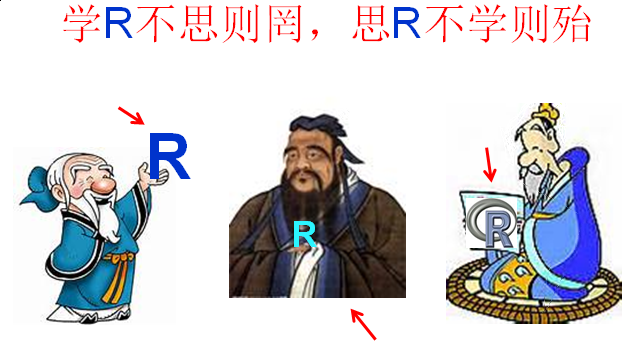
\includegraphics[width=.8\textwidth]{Confucious} \caption
  {Learning \R{} without thinking it makes one confused; thinking \R{}
  without learning it makes one shallow --- Chenshun Lin, the chair of the
  lightning talk sessions, added \R{} to a famous quote by Confucious and
  turned it to a hilarious pun.}
\end{figure}

The two-day event was a great success and we got many positive feedback
messages from participants after the conference. We will further devote our
future effort on:

\begin{itemize}

  \item organizing more R meetings to meet the growing demand of R users in
  China;

  \item promoting statistics and data analysis in the industry;

  \item interacting with different fields, such as e-commerce, through more
  and advanced applications of R.

\end{itemize}

The conference summary and slides are freely available at \url
{http://cos.name/chinar/chinar-2013/} (in Chinese). We would like to thank
the School of Statistics and the Center for Applied Statistics of RUC for
their consistent support for the Chinese R Conference. We are also grateful
to Prof Hansheng Wang for his encouragement and generous help. We appreciate
the tremendous help of all student volunteers from RUC and COS. We look
forward to the next R conference in China and warmly welcome more people to
attend it. Inquiries and suggestions can be sent to \email
{chinar-committee@cos.name}.

The conference committee consists of Tao Gao (Chair), Yu Chen (Vice Chair),
Taiyun Wei, Sen Chen, Jianchong Su, Yanping Chen, Sizhe Liu, Yihui Xie,
Manqi Xie, Zhanhang Xiao, Yishuo Deng, Yixuan Qiu, Yan Chen, Jing Leng.

\address{Jing Leng\\
  School of Statistics, Renmin University of China\\
  Beijing, China P. R.}\\
\email{jing.leng@cos.name}

\address{Jingjing Guan\\
  College of Business, City University of Hong Kong\\
   Hong Kong SAR}\\
\email{jingjing.guan@cos.name}
